\documentclass[]{elsarticle} %review=doublespace preprint=single 5p=2 column
%%% Begin My package additions %%%%%%%%%%%%%%%%%%%
\usepackage[hyphens]{url}



\usepackage{lineno} % add
\providecommand{\tightlist}{%
  \setlength{\itemsep}{0pt}\setlength{\parskip}{0pt}}

\bibliographystyle{elsarticle-harv}
\biboptions{sort&compress} % For natbib
\usepackage{graphicx}
\usepackage{booktabs} % book-quality tables
%%%%%%%%%%%%%%%% end my additions to header

\usepackage[T1]{fontenc}
\usepackage{lmodern}
\usepackage{amssymb,amsmath}
\usepackage{ifxetex,ifluatex}
\usepackage{fixltx2e} % provides \textsubscript
% use upquote if available, for straight quotes in verbatim environments
\IfFileExists{upquote.sty}{\usepackage{upquote}}{}
\ifnum 0\ifxetex 1\fi\ifluatex 1\fi=0 % if pdftex
  \usepackage[utf8]{inputenc}
\else % if luatex or xelatex
  \usepackage{fontspec}
  \ifxetex
    \usepackage{xltxtra,xunicode}
  \fi
  \defaultfontfeatures{Mapping=tex-text,Scale=MatchLowercase}
  \newcommand{\euro}{€}
\fi
% use microtype if available
\IfFileExists{microtype.sty}{\usepackage{microtype}}{}
\ifxetex
  \usepackage[setpagesize=false, % page size defined by xetex
              unicode=false, % unicode breaks when used with xetex
              xetex]{hyperref}
\else
  \usepackage[unicode=true]{hyperref}
\fi
\hypersetup{breaklinks=true,
            bookmarks=true,
            pdfauthor={},
            pdftitle={Urban and socio-economical correlates of property price fluctuaction, an Dublin case study},
            colorlinks=false,
            urlcolor=blue,
            linkcolor=magenta,
            pdfborder={0 0 0}}
\urlstyle{same}  % don't use monospace font for urls

\setcounter{secnumdepth}{0}
% Pandoc toggle for numbering sections (defaults to be off)
\setcounter{secnumdepth}{0}
% Pandoc header
\usepackage{float}
\usepackage{booktabs}
\usepackage{array}
\usepackage{tabu}
\floatplacement{figure}{H}



\begin{document}
\begin{frontmatter}

  \title{Urban and socio-economical correlates of property price fluctuaction, an
Dublin case study}
    
  \begin{abstract}
  This is the abstract.
  \end{abstract}
  
 \end{frontmatter}

\hypertarget{introduction}{%
\section{Introduction}\label{introduction}}

To acquire a property is one of the most important achievement that
individuals are seeking. It provides not only a housing security but
also the feeling of being a landowner. However the access to the status
of landowner is complicated because buying a property is the most
expensive spending of in a lifetime. For this reason understanding the
factors which are explaining how property prices evolve is a necessity.

Due to its geographic, economic and political situation, Ireland in
general and Dublin in particular saw important changes in property
prices in the last ten years. From a economic boom known as the ``Celtic
tiger'' in the 2000's, Ireland were deeply impacted by the 2007 economic
crisis. With an expected GDP growth of 4\% for 2019, property prices are
back to their highest. Whereas this grow is moderated in Irish mainland,
its capital Dublin is at the center of a housing crisis. Because of
factors including Irish economic wealth, the presence of tech companies
European headquarters such as Facebook or Google and the historic
configuration of the city which low population density structure and
underdeveloped public transportation, property prices became
unaffordable to most of Irish families.

In this paper we want to identify the spatio-temporal factors that
influenced the evolution of Dublin property prices. More precisely we
want to highlight not only macro economical influences such as GDP but
also the presence of economical landmarks such as tech companies
headquarters and public transportation system on property prices
evolution.

\hypertarget{method}{%
\section{Method}\label{method}}

Since the 1st January 2010, under the Property Services (Regulation)
Act, all individuals acquiring a property in Ireland has to declare it
to Property Services Regulatory Authority (PSRA). It includes Date of
Sale, Price and Address of all residential properties purchased in
Ireland as declared to the Revenue Commissioners for stamp duty purposes
(https://propertypriceregister.ie). It must be noticed that data is
filed electronically by persons doing the conveyancing of the property
on behalf of the purchaser and errors may occur when the data is being
filed. In order to evaluate the spacial distribution of the property
sold, a geocoding from the filled addresses to GPS coordinated was
performed using the OpenStreetMap API.

\begin{table}[!h]

\caption{\label{tab:dublin-sample-size}Size of the PSRA database for properties sold in Dublin County per year since 2010 aftering filtering the orignal database.}
\centering
\fontsize{8}{10}\selectfont
\begin{tabular}{rr}
\toprule
year & n\\
\midrule
2010 & 4819\\
2011 & 3745\\
2012 & 4910\\
2013 & 5577\\
2014 & 832\\
2015 & 9657\\
2016 & 10731\\
2017 & 11991\\
2018 & 10395\\
\bottomrule
\end{tabular}
\end{table}

By focusing on the property sold in Dublin, 111155 entries were recorded
since 2010. After having filtered properties not corresponding to
houses, properties for which address was not possible to geocode,
artifacts in geocodes and aberrant value in sales price. From the
self-reported database, 62657 properties sold in Dublin between
2010-01-01 and 2018-11-30 was geocoded.

\hypertarget{results}{%
\section{Results}\label{results}}

The average properties price is €330,364 euros (SD = €180,448). In order
to remove potential human errors and outliers, prices higher or lower
than 1 SD were removed from the original dataset.

\begin{figure}[H]
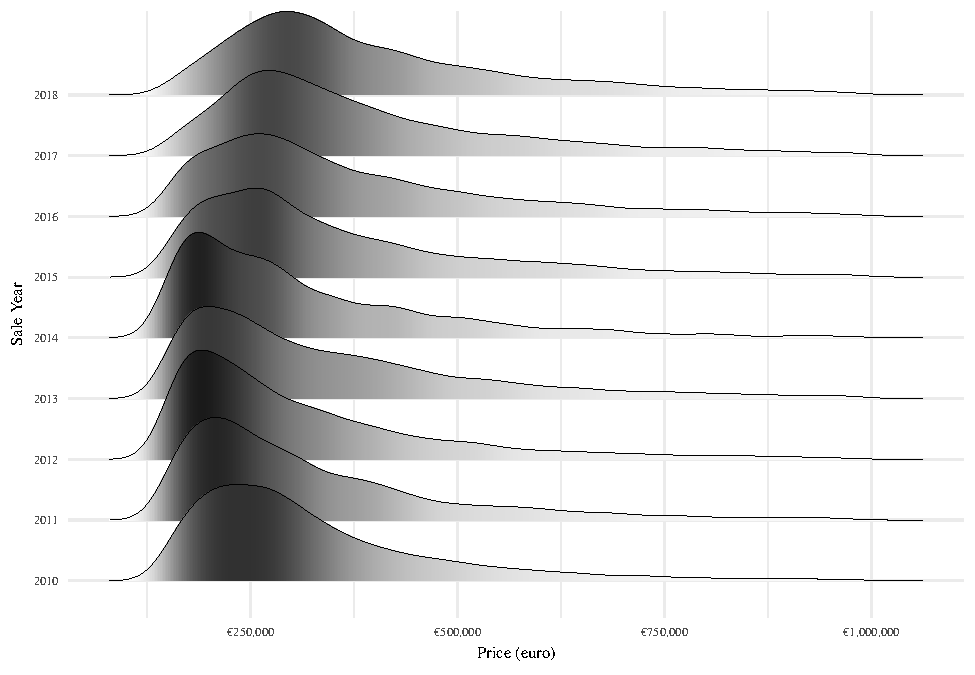
\includegraphics{property_price_paper_new_files/figure-latex/distrib-plot-1} \caption{Distribution of the PSRA database (filtered).}\label{fig:distrib-plot}
\end{figure}

The density of housing prices distribution reveals a slight decrease
with a minimum in 2013 and 2014 which corresponds to the repercussion of
the Irish economic crisis.

\begin{figure}[H]
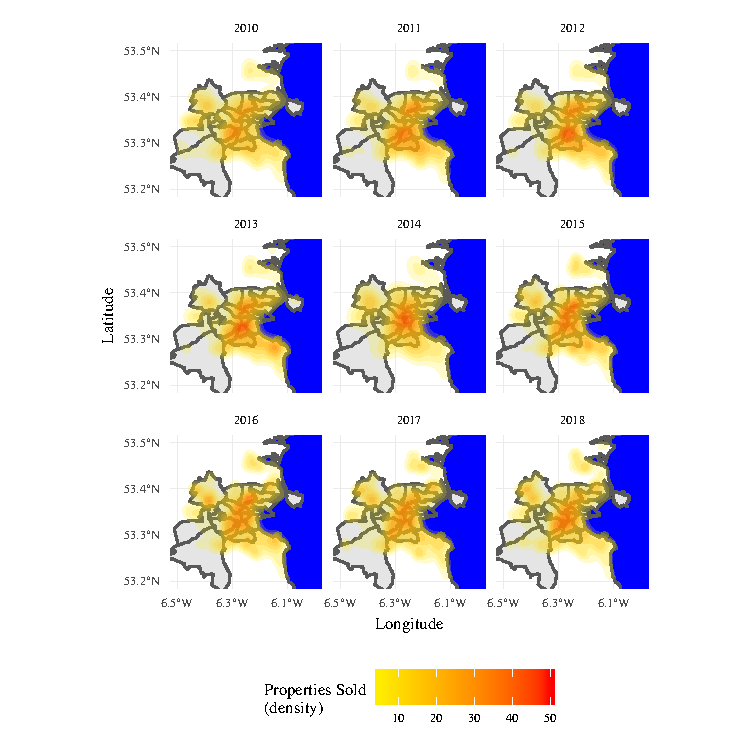
\includegraphics{property_price_paper_new_files/figure-latex/density-plot-1} \caption{Geographical density of the PSRA database (filtered).}\label{fig:density-plot}
\end{figure}

The distribution of properties sold in Dublin indicates that most of the
properties sold are located around Dublin 6 and Dublin 6 West districts
for every year investigated. However in order to evaluate and to predict
the distribution of housing prices, a generalized additive model with
model soap film smoother (Wood, Bravington and Hedley, 2008) is computed
on the Dublin area. Soap film smoother are constructing a 2-D smooth
prediction of non-linear parameters such as latitude and longitude. The
smooths are designed to fit geographical models including coastal
boundaries.

In order to model the distribution of properties, a Generalized Additive
Model using Gaussian scale family for Soap film smooths was calculated
to fit the price of properties sold according to their GPS coordinates.
The result indicates that 20.3\% of property prices is explained by
property localisation (\emph{F}(62657,60.95) = 214.97; \emph{p}
\textless{} 0.001).

\begin{figure}[H]
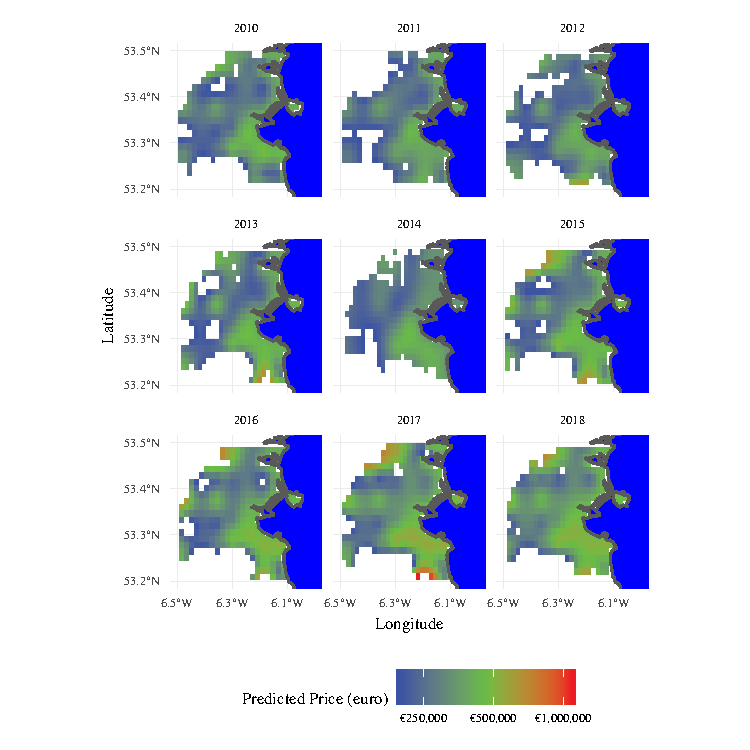
\includegraphics{property_price_paper_new_files/figure-latex/gam-year-plot-1} \caption{Prediction of property price according the GAM model. Prediction too far from the actual data were removed to avoid unrealistic extrapolation.}\label{fig:gam-year-plot}
\end{figure}

The Generalized Additive Model reveal not only high prices located on
the coast of Dublin (i.e Dublin 4 and Dun Laoghaire) but also a spot in
Dublin 7 which was unexpected.

\hypertarget{prediction-of-property-price-using-xgboost}{%
\subsection{Prediction of property price using
XGBoost}\label{prediction-of-property-price-using-xgboost}}

In order to increase the prediction accuracy of the Generalized Additive
Model an XGBoost regression was performed on 195 geographic, economic
and social features.

\hypertarget{geographical-feature-extraction}{%
\subsubsection{Geographical feature
extraction}\label{geographical-feature-extraction}}

Open Street map is a collaborative project which aims to create and
provide access to free editable maps of the world. Open Street Map
combines information about more than 1177 features including road
information and building information to categorize amenities, leisure or
tourism structure for example. Among the 1177 features only 143 contain
data for the Dublin Area (See list of Open Street Map features in
Appendix 1). In order to process the XGBoost regression the distance
between each property and the closest point corresponding to each of the
143 relevant Open Street Map.

\begin{figure}[H]
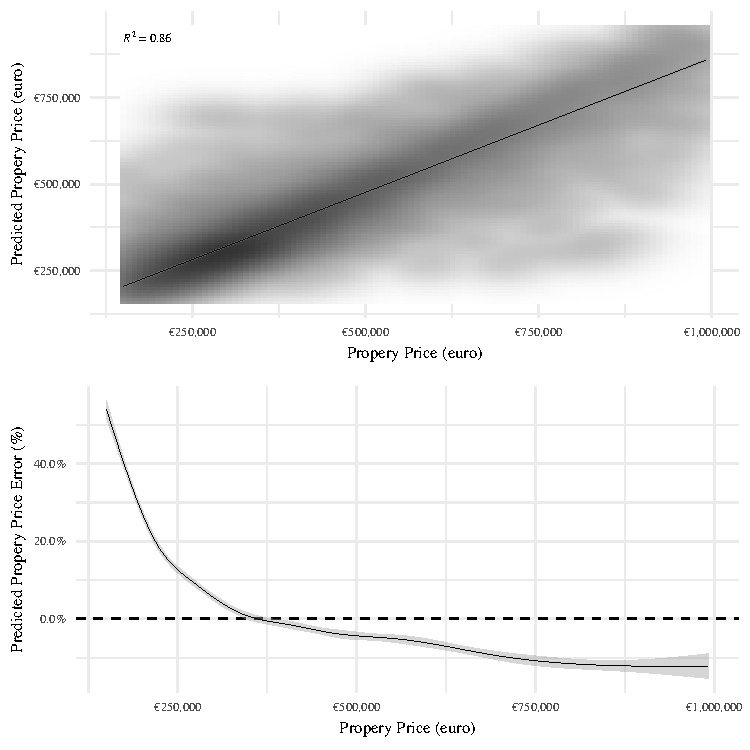
\includegraphics{property_price_paper_new_files/figure-latex/OSM-features-xgb-1} \caption{Property price prediction accuracy (top) and Property price prediction error (bottom) using geographical features with XGBoost.}\label{fig:OSM-features-xgb}
\end{figure}

The prediction accuracy using the XGBoost algorithm reaches a very high
level of 86\% (\(R^2 = .86\), \(F(1, 10387) = 62,556.39\),
\(p < .001\)). Whereas they constitute half of the houses sold, prices
lower than €300.000 are the most difficult to predict because. A
possible explanation is the absence of a recurrent pattern in
geographical features for these houses.

\begin{table}[!h]

\caption{\label{tab:OSM-features-table}Open Street Map features importance (higher than 1\%).}
\centering
\fontsize{8}{10}\selectfont
\begin{tabular}{>{\raggedright\arraybackslash}p{1in}>{\raggedright\arraybackslash}p{3in}l}
\toprule
Feature Category & Feature Type & Importance\\
\midrule
amenity & embassy & 17.0\%\\
natural & grassland & 6.0\%\\
route & bus & 2.0\%\\
power & line & 2.0\%\\
boundary & administrative & 2.0\%\\
barrier & wall & 2.0\%\\
cycleway & lane & 2.0\%\\
amenity & bar & 1.0\%\\
place & island & 1.0\%\\
boundary & political & 1.0\%\\
boundary & historic & 1.0\%\\
cutting & yes & 1.0\%\\
barrier & full-height & 1.0\%\\
area & yes & 1.0\%\\
route & road & 1.0\%\\
place & locality & 1.0\%\\
tunnel & yes & 1.0\%\\
junction & roundabout & 1.0\%\\
cycleway & track & 1.0\%\\
barrier & hedge & 1.0\%\\
route & ferry & 1.0\%\\
\bottomrule
\end{tabular}
\end{table}

By analyzing their importance, the most relevant geographical features
to predict housing prices are the presence of an embassy (17\%) and the
presence of natural grasslands such as parks and gardens (6\%).

\hypertarget{economic-and-social-feature-extraction}{%
\subsubsection{Economic and social feature
extraction}\label{economic-and-social-feature-extraction}}

The results of Irish 2011 census consultation is accessible through the
All-Island Research Observatory and can be mapped over Ireland small
area boundaries which are fraction of Irish Electoral Division map. The
social features extracted are corresponding to population information,
religion, carers and health. Economic features correspond to the type of
each small area including the proportion of housing type, rooms number,
occupancy and tenure per small area. Each property is then associated to
the value corresponding to its small area.

\begin{figure}[H]
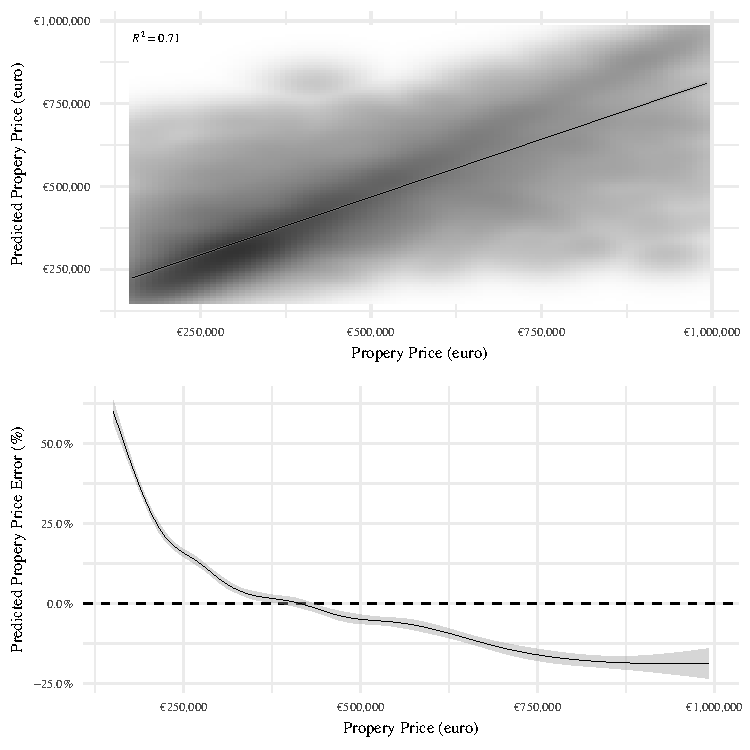
\includegraphics{property_price_paper_new_files/figure-latex/census-features-xgb-1} \caption{Property price prediction accuracy (top) and Property price prediction error (bottom) using socio-economic features with XGBoost.}\label{fig:census-features-xgb}
\end{figure}

Whereas the prediction accuracy using the XGBoost algorithm with
socio-economic features is lower than the prediction with geographical
data, result show an accuracy of 71\% (\(R^2 = .71\),
\(F(1, 10387) = 24,916.00\), \(p < .001\)). In a similar way than for
geographical feature prediction, houses prices lower than €300.000 led
to the highest prediction errors.

\begin{table}[!h]

\caption{\label{tab:census-features-table}Irish census features importance (higher than 1\%).}
\centering
\fontsize{8}{10}\selectfont
\begin{tabular}{>{\raggedright\arraybackslash}p{1in}>{\raggedright\arraybackslash}p{3in}l}
\toprule
Feature Category & Feature Type & Importance\\
\midrule
housing rooms & \% 8 or more Rooms (Households) & 29.4\%\\
religion & \% No Religion & 5.3\%\\
population & \% Age 0 - 14 & 4.2\%\\
general health & \% Very Good & 3.4\%\\
housing rooms & \% 6 Rooms (Households) & 3.1\%\\
population & \% Age 80 Plus & 2.9\%\\
housing rooms & \% 5 Rooms (Households) & 2.2\%\\
religion & \% Other Catholic & 2.1\%\\
religion & \% No Answer & 2.0\%\\
housing rooms & \% 3 Rooms (Households) & 2.0\%\\
housing tenure & \% Social Rented & 2.0\%\\
housing rooms & \% 7 Rooms (Households) & 1.9\%\\
housing tenure & \% Owner Occupier No Mortgage (Households) & 1.9\%\\
disabilty age group & \% Persons with a disability aged 0 - 14 & 1.8\%\\
housing tenure & \% Private Rented & 1.8\%\\
housing tenure & \% Owner Occupier with Mortgage (Households) & 1.7\%\\
religion & \% Roman Catholic & 1.7\%\\
general health & \% Good & 1.7\%\\
population & \% Age 45 - 64 & 1.6\%\\
housing rooms & \% 4 Rooms (Households) & 1.6\%\\
disabilty age group & \% Persons with a disability aged 25 - 44 & 1.6\%\\
disabilty age group & \% Persons with a disability aged 65 Plus & 1.6\%\\
general health & \% Bad & 1.6\%\\
housing rooms & \% 1 Room (Households) & 1.4\%\\
population & \% Age 15 - 24 & 1.3\%\\
carers & \% Provides No Care & 1.3\%\\
population & \% Age 25 - 44 & 1.3\%\\
population & \% Female & 1.2\%\\
disabilty age group & \% Persons with a disability aged 45 - 64 & 1.2\%\\
housing occupancy & \% Occupied/HS With ususal Residents & 1.2\%\\
population & \% Age 65 Plus & 1.2\%\\
housing type & \% House/Bungalow & 1.1\%\\
\bottomrule
\end{tabular}
\end{table}

The most important socio-economical feature are the proportion of large
houses in the small area (29.4\%). It appears that areas in which the
proportion of people reporting having no religion also influences the
model (5.3\%) as well as the proportion of children (4.2\%) and the
proportion of healthy inhabitant in the area (3.4\%).

\hypertarget{conclusion}{%
\section{Conclusion}\label{conclusion}}

The evolution of housing prices is a real problem in most of European
capitals and specially in Dublin. Given their significant increase,
houses are less and less affordable for individuals. Using Generalized
Additive Model we were able to identify the influence of property
locations based in Dublin on their actual sale price. Houses actual
location is the main factor influencing houses prices but it is
difficult to know why some areas are more valuable than others. By
preforming a feature analysis with geographical and socio-economical
variable it is possible to evaluate and predict the potential price of a
house. Indeed features such as presences of embassies or parks are
criteria that influence significantly the price of houses. Similarly,
the characteristics of inhabitants in the area such as religion, health
and age is correlated to the evolution of housing prices. These results
allow to understand why an area have higher prices than others.

\hypertarget{appendix}{%
\section{Appendix}\label{appendix}}

\begin{table}[t]

\caption{\label{tab:all-OSM-features}Relevant Open Street Map features for dublin area.}
\centering
\fontsize{8}{10}\selectfont
\begin{tabu} to \linewidth {>{\raggedright\arraybackslash}p{1in}>{\raggedright}X}
\toprule
Feature Category & Feature Type\\
\midrule
amenity & bar, college, school, university, bicycle parking, fuel, parking, community centre, bench, embassy, police, prison, recycling\\
barrier & city wall, ditch, fence, guard rail, hedge, kerb, retaining wall, wall, block, bollard, chain, full-height turnstile, gate, jersey barrier, yes\\
boundary & administrative, historic, political, postal code, protected area\\
building & apartments, house, residential, commercial, industrial, retail, hospital, university, yes\\
highway & motorway, trunk, secondary, tertiary, unclassified, residential, service, motorway link, trunk link, secondary link, tertiary link, pedestrian, track, road, footway, steps, path, cycleway\\
cycleway & lane, opposite, opposite lane, track, share busway, shared lane\\
busway & lane\\
highway & proposed, construction\\
junction & roundabout\\
historic & yes\\
landuse & commercial, construction, industrial, residential, retail, farmland, grass, military, railway, recreation ground, religious\\
leisure & nature reserve, park, slipway, sports centre, stadium, track\\
man made & breakwater, crane, embankment, groyne, pier, pipeline\\
natural & wood, tree row, scrub, grassland, water, beach, coastline, ridge, cliff\\
place & district, county, city, suburb, island, locality\\
power & cable, line, minor line, portal\\
line & busbar\\
public transport & platform, stop area\\
railway & abandoned, disused, rail, tram, platform\\
bridge & yes\\
cutting & yes\\
electrified contact & line\\
embankment & yes\\
service & crossover, siding, spur, yard\\
tunnel & yes\\
usage & main\\
route & bicycle, bus, ferry, hiking, power, road, train, tram\\
shop & paint, kitchen,\\
sport & badminton, equestrian, gaelic games, rugby union, running\\
tourism & artwork, zoo\\
waterway & river, riverbank, stream, canal, drain, ditch, weir, lock gate\\
source & survey\\
area & yes\\
covered & yes\\
disused & yes\\
tidal & yes\\
\bottomrule
\end{tabu}
\end{table}

\begin{table}[t]

\caption{\label{tab:all-census-features}Relevant Irish census features for dublin area.}
\centering
\fontsize{8}{10}\selectfont
\begin{tabu} to \linewidth {>{\raggedright\arraybackslash}p{1in}>{\raggedright}X}
\toprule
Feature Category & Feature Type\\
\midrule
carers & \% Provides No Care,                          
 \% 1-19 hours unpaid PW,                     
 \% 20-49 hours unpaid PW,                     
 \% 50+ hours unpaid PW,                      
 \% Total Care Providers\\
disabilty\_age\_group & \% Persons with a disability aged 0 - 14,      
 \% Persons with a disability aged 15 - 44,    
 \% Persons with a disability aged 25 - 44,   
 \% Persons with a disability aged 45 - 64,    
 \% Persons with a disability aged 65 Plus,   
 \% Total persons with a disability\\
general\_health & \% Very Good,                                
 \% Good,                                     
 \% Fair,                                     
 \% Bad,                                       
 \% Very Bad\\
housing\_occupancy & \% Occupied/HS With ususal Residents,         
 \%  Unoccupied/HS Without Ususal Residents\\
housing\_rooms & \% 1 Room (Households),                      
 \% 2 Rooms (Households),                      
 \% 3 Rooms (Households),                     
 \% 4 Rooms (Households),                      
 \% 5 Rooms (Households),                     
 \% 6 Rooms (Households),                      
 \% 7 Rooms (Households),                     
 \% 8 or more Rooms (Households),              
 \% Total (Households)\\
housing\_tenure & \% Owner Occupier with Mortgage (Households),
 \% Owner Occupier No Mortgage (Households),   
 \% Private Rented,                           
 \% Social Rented,                             
 \% Rented Free of Rent (Households),        
 \% Total (Households)\\
housing\_type & \% House/Bungalow,                           
 \% Flat/Apartment/BedSit,                     
 \% Caravan/Mobile home/Temperory\\
population & \% Male,
 \% Female,
 \% Age 0-14
 \% Age 15 - 44,    
 \% Age 25 - 44,   
 \% Age 45 - 64,    
 \% Age 65 Plus,
 \% Age 15 - 64, 
 \% Age 80 Plus\\
religion & \% Roman Catholic,
\% Other Catholic,
\% Other Religion,
\% No Religion,
\% No Response\\
\bottomrule
\end{tabu}
\end{table}

\hypertarget{references}{%
\section*{References}\label{references}}
\addcontentsline{toc}{section}{References}

\end{document}


